\documentclass[11pt]{article}

\usepackage{subfigure}
\usepackage{pgfplots}
\usepackage[top=3cm,left=3cm,right=3cm,bottom=3cm]{geometry}
% Scriptsize axis style.
\pgfplotsset{every axis/.append style={tick label style={/pgf/number format/fixed},font=\scriptsize,ylabel near ticks,xlabel near ticks,grid=major}}

\begin{document}
\begin{figure}[t!]
	\centering
	\subfigure[Logistic sigmoid activation function.]{
    		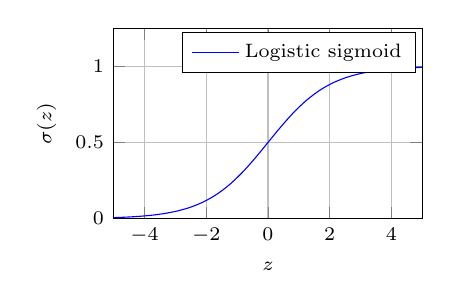
\begin{tikzpicture}
			\begin{axis}[width=5.5cm,height=4cm,ylabel=$\sigma(z)$,xlabel=$z$,ymin=0,ymax=1.25,xmin=-5,xmax=5]
				\addplot[blue,smooth] {1/(1+exp(-x))};
				\addlegendentry{Logistic sigmoid}
			\end{axis}
		\end{tikzpicture}
	}
	\subfigure[Hyperbolic tangent activation function.]{
		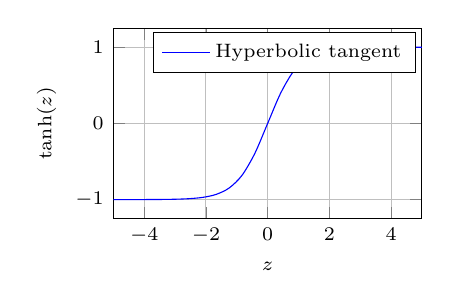
\begin{tikzpicture}
			\begin{axis}[width=5.5cm,height=4cm,ylabel=$\tanh(z)$,xlabel=$z$,ymin=-1.25,ymax=1.25,xmin=-5,xmax=5]
				\addplot[blue,smooth] {tanh(x)};
				\addlegendentry{Hyperbolic tangent}
			\end{axis}
		\end{tikzpicture}
	}\\
	\subfigure[Logistic sigmoid activation function.]{
    		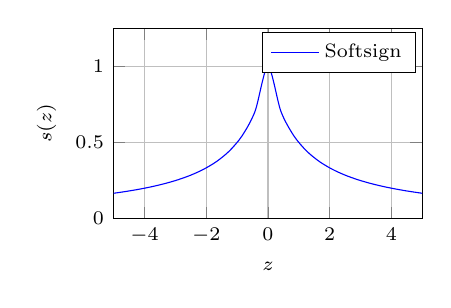
\begin{tikzpicture}
			\begin{axis}[width=5.5cm,height=4cm,ylabel=$s(z)$,xlabel=$z$,ymin=0,ymax=1.25,xmin=-5,xmax=5]
				\addplot[blue,smooth] {1/(1 + abs(x))};
				\addlegendentry{Softsign}
			\end{axis}
		\end{tikzpicture}
	}
	\subfigure[Rectified hyperbolic tangent activation function.]{
		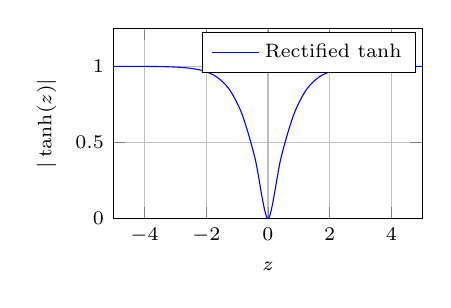
\begin{tikzpicture}
			\begin{axis}[width=5.5cm,height=4cm,ylabel=$|\tanh(z)|$,xlabel=$z$,ymin=0,ymax=1.25,xmin=-5,xmax=5]
				\addplot[blue,smooth] {abs(tanh(x))};
				\addlegendentry{Rectified $\tanh$}
			\end{axis}
		\end{tikzpicture}
	}
    	\caption[Sigmoidal activation functions.]{Common used activation functions include the logistic sigmoid $\sigma(z)$ and the hyperbolic tangent $tanh(z)$. More recently used activation functions are the softsign and the rectified hyperbolic tangent.}
    	\label{fig:sigmoid-tanh}
\end{figure}
\end{document}
